\documentclass[11pt,a4paper,oneside]{memoir}

% Packages
\usepackage[a4paper,margin=2.5cm, top=1.5in, bottom=1.5in]{geometry}
\usepackage{graphicx}
\usepackage{enumerate}
\usepackage{amsmath}
\usepackage{amssymb}
\usepackage{amsfonts}
\usepackage{amsthm}
\usepackage{tikz}
\usepackage{float}
\usepackage[T1]{fontenc}
\usepackage[
    colorlinks=true,
    %linkcolor=blue, urlcolor=blue, citecolor=blue % pdf
    linkcolor=black, urlcolor=black, citecolor=black % print
]{hyperref}

\usetikzlibrary{positioning}
\usetikzlibrary{arrows.meta}

% Look for images under the .images/ dir
\graphicspath{ {./images/} }
% Specifiy stype for bibliography
\bibliographystyle{abbrv}

% Theorem and Proposition styling
\theoremstyle{plain}
% Reset theorem numbering for each chapter
\newtheorem{thm}{Theorem}[chapter]
% Reset definition numbering for each chapter
\newtheorem{prop}[thm]{Proposition}
% Reset definition numbering for each chapter
\newtheorem{lem}[thm]{Lemma}

% Definition and Example styling
\theoremstyle{definition}
% Definition numbers are dependent on theorem numbers
\newtheorem{defn}[thm]{Definition}
% Example numbers are dependent on theorem numbers
\newtheorem{exmp}[thm]{Example}

\newcommand{\mmod}[1]{\ (\mathrm{mod}\ #1)}

\begin{document}

% -------------- TITLE PAGE --------------
\begin{titlingpage}
    \centering
 
        \Huge
        \parbox{10cm}{\begin{center}{\scshape \textbf{Chaos in Topological Dynamical Systems}}\end{center}}
             
        \vspace{1.25cm}

        \large
        by

        \vspace{1cm}
        
        \LARGE
        {\scshape \textbf{Fraser Robert Love}}
             
        \vspace{1.5cm}
             
        \large
        School of Mathematics and Statistics\\
        University of St Andrews\\

        \vfill

        {\large \today\par}
 \end{titlingpage}
% ------------ TITLE PAGE END ------------

% Set correct spacing between lines
\OnehalfSpacing

\noindent\textit{I certify that this project report has been written by me, is a record of work carried out by me, and is essentially different from work undertaken for any other purpose or assessment.}

\begin{center}

\includegraphics[width=1.3cm]{signature}
\end{center}

\vspace{1cm}

\begin{abstract}
    \noindent A topological dynamical system is comprised of a continous mapping acting on an underlying compact metric space. These systems often give rise rise to complex and chaotic behaviour. This project explores various definitions of chaos applied to topological dynamical systems and the properites they hold. Specifically we will cover Devaney chaos, Li and Yorke chaos and topological chaos and how these definitions apply to topological dynamical systems on the interval, the unit circle, in sequence space and on compact countable sets. We shall encounter a wide variety of chaotic behaviors, such as topological transitivity, sensitive dependence on initial coditions, the density of periodic points, scrambled sets and topological entropy. Finally the text shall conclude by characterising various chaotic systems and compairing the various definitions of chaos.
\end{abstract}

\newpage
\tableofcontents

\chapter{An Introduction to Topological Dynamics}
This aim of this text is to introduce the reader to topological dynamical systems and explore the various interpretations of chaos and their consequences. We shall be tackling chaos through the lense of topology and topological dynamical systems. A discrete dynamical system is defined by a metric space with a corresponding continuous function, mapping the metric space to itself. The function itself is termed a map or mapping whereby points in the underlying metric space are mapped to other points in the set by the application of this function. Topological dynamical systems themselves are a subset of discrete dynamical systems, with the extra requirement that the underlying metric space be compact (i.e.\ complete and totally bounded). This extra condition for compactness is useful for investigating the limiting behavior of the set of iterates of the map as it is repeatedly iterated to infinity; a relevant feature in the study of chaos. The term chaos itself, specifically deterministic chaos, has various definitions in mathematics and was first coined by Li and Yorke in their ubiquitious paper `Period Three Imples Chaos' \cite{li-yorke}. These numerous definitions provide differing constituents to chaos namely: topological transitivity, existence of a dense orbit, the density of periodic points, existence of an uncountable scrambled set and sensitive dependence on initial conditions. Hence topological dynamical systems can be chaotic according to one interpretation but not another. We shall aim to compare these definitions and understand their consequences, providing examples to topological dynamical systems that exhibit each type of chaos. Specifically we shall be restrict our attention to three compact metric spaces, closed intervals, the unit circle, and sequence space. This text assumes the reader to be a capable student of pure mathematics with a basic understanding of topology and analysis. The focus of this text is mainly topological; for the sake of brevity content from related areas of ergodic theory, group theory, etc.\ are excluded.

This chapter will briefly review some relevant results from topology before introducing ideas central to topological dynamics and the study of chaos in topological dynamical systems. We shall also introduce some popular topological dynamical systems that exhibit chaos, which we will be examining throughout this text. Subsequently, in Chapter 2 we will introduce notions of comparing and equivalating topological dynamical systems using the framework of topological conjugacy and symbolic dynamics. Here we will use these powerful results to prove topological results for the well k   nown tent map and logistic map using topologically conjugate maps. Furthermore, we shall begin our study of chaos via Sharkovsky's theorem. In Chapter 3 we will study the three various interpretations of chaos from called Devaney chaos, Li and Yorke chaos, and topological chaos, analysing examples of topological dynamical systems which statisfy each definition. We shall look at the various properties topological dynamical systems require to be considered chaotic and compare the various definitions. Finally in Chapter 4 we will explore the consequences of chaos and characterise the interesting behavior of topological dynamical systems.

\section{Topological Dynamical Systems and Discrete Dynamics} \label{sec:topological-dynamical-systems}
We shall start this chapter by giving the definition of a topological dynamical system, including some important defintions from topology and introducing some preliminary definitions from discrete dynamics. We shall refer back to these definitions constantly for the remainder of this text. Furthermore, prominent examples of topological dynamical systems will be presented. The reader should remember these examples as they will be integral to understanding several propositions in later chapters. Note that the definitions and results in this section apply generally to continuous maps, however have been formulated in terms of topological dynamical systems for clarity and precision. Beginning, we shall introduce some preliminary definitions from topology.

\begin{defn}[Dense Set] \label{defn:dense}
    Let $(Z, d)$ be a metric space and $X, Y \subseteq Z$ where $X \subseteq Y$. The set $X$ is \emph{dense} in $Y$ if $\overline{X} = Y$, i.e.\ if for every $x \in Y$ there exits an open neighbourhood $U$ of $x$ with $y \in U$ such that $y \in X$.
\end{defn}

\begin{defn}[Compact  Space] \label{defn:compact}
    A metric space $(X, d)$ is \emph{compact} if every open cover $\mathcal{U}$ of $X$ has a finite subcover $\left\lbrace U_{i(1)}, U_{i(2)}, \cdots, U_{i(n)} \right\rbrace \subseteq \mathcal{U}$, i.e.\ if $\left\lbrace U_i \right\rbrace_{i\in I}$ is a collection of open subsets of $X$, where $X \subseteq \bigcup_{i \in I}U_i$ then there exists a finite subcollection $\left\lbrace U_{i(1)}, U_{i(2)}, \cdots, U_{i(n)} \right\rbrace \subseteq \mathcal{U}$ such that $X \subseteq \bigcup_{j = 1}^{n}U_{i(j)}$. Furthermore, a metric space is compact if and only if it is complete and totally bounded.
\end{defn}

Note that on $\mathbb{R}$ with the standard metric, all closed intervals are compact. Now since we now have a notion of what it means for a metric space to be compact we can now define the main object we shall be studying in this paper, the topological dynamical system.

\begin{defn}[Topological Dynamical System] \label{defn:topological-dynamical-system}
    Let $X$ be a non-empty compact metric space. A \emph{topological dynamical system} denoted $(X, f)$ is given by a continuous map $f: X \to X$. The system starts at an initial point $x \in X$ and evolves through successive iterations of the map $f$. After $k \in \mathbb{N}$ iterations of $f$, the system can be described by $f^n := f \circ f \circ \cdots \circ f$, where $f$ is mapped to the point $f^n(x)$. By convention we take $f^0$ to be the identity map.
\end{defn}

Having defined a topological dynamical system, we can now characterise the discrete dynamics of the underlying map through the following definitions.

\begin{defn}[Orbit] \label{defn:orbit}
    Let $(X, f)$ be a topological dynamical system. The \emph{orbit} or \emph{forward orbit} of a point $x \in X$ under $f$ is the set $\mathcal{O}_f(x) = \mathcal{O}^+_f(x) = \lbrace f^n(x) : n \geq 0 \rbrace = \lbrace x, f(x), f^2(x), \cdots \rbrace$ of iterates of $x$ under the map $f$. If $f$ is a homeomorphism (i.e $f^{-1}$ exists and is continuous) then the \emph{backward orbit} of $x$ under $f$ is similarly defined as $\mathcal{O}^-_f(x) = \lbrace f^n(x) : n \leq 0 \rbrace = \lbrace x, f^{-1}(x), f^{-2}(x), \cdots \rbrace$.
\end{defn}

Note that in this text, unless otherwise stated, the term, orbit, will simply refer to the forward orbit, as we will mostly be dealing with forward dynamics. An interesting property of topological dynamical systems is the existence of a dense orbit. From Definition \ref{defn:dense} we note an orbit $\mathcal{O}_f(x)$ of $f$ is said to be dense in $X$ if for every $x \in X$ and $\varepsilon > 0$ there exits a $n \in \mathbb{N}$ such that $d(x_n, x) \leq \varepsilon$.

\begin{defn}[Periodic Point, Cycle] \label{defn:periodic-point}
    Let $(X, f)$ be a topological dynamical system. A point $x \in X$ is \emph{fixed} if $f(x) = x$ and \emph{periodic} if $f^n(x) = x$ for some $n \in \mathbb{N}$. The \emph{period} of a point $x$ is the least positive integer $k$ such that $f^k(x) = x$. If $x$ has a period of $k$ we say that $x$ is a \emph{period-$k$} point. The set of all period-$k$ points of $f$ is denoted by $\text{Per}_k(f)$ and the set of all periodic points of $f$ is denoted $\text{Per}(f)$. Moreover, $f^n(x) = x \iff n = lk$, for some $l \in \mathbb{N}$. The orbit $\mathcal{O}_f(x) = \lbrace x, f(x), \cdots, f^{k-1}(x) \rbrace$ of a periodic point is a finite set of unique points, called a \emph{perodic orbit} of period $k$ or simply a \emph{k-cycle}.
\end{defn}

In most topological dynamical systems only a small subset of points are periodic. Most often a larger set of points either enter a periodic orbit after a certain number of iterations of $f$ or converge asymptotically to a periodic orbit, leading us directly into the following defintions.

\begin{defn}[Eventually Periodic, Asymptotically Periodic] \label{defn:eventually-asymptotically-periodic}
    Let $(X, f)$ be a topological dynamical system. A point $x \in X$ is \emph{eventually periodic} of period $k$ if the point $x$ is not periodic and there exists a $n > 0$ such that $f^{k+i}(x) = f^i(x)$, for $i \geq n$. The point $x \in X$ is \emph{asymptotically periodic} to a periodic point $p \in X$ if $\lim_{n \to \infty} d(f^n(x), f^n(p)) = 0$.
\end{defn}

\begin{prop} \label{prop:eventually-periodic-implies-periodic}
    Let $(X, f)$ be a topological dynamical system. If $f$ is an invertible map, then every eventually periodic point is periodic.
    \begin{proof}
        Suppose $x \in X$ is eventually periodic of period $k$ in $f$. Then $f^{k + i}(x) = f^i(x)$ for some $n > 0$. By applying $i$ iterations of $f^{-1}$ we obtain, $f^{-i} \circ f^{k + i}(x) = f^{-i} \circ f^{i}(x) \implies f^k(x) = x$. Hence $x$ is periodic with period $k$.
    \end{proof}
\end{prop}

When studying chaos in topological dynamical systems it can be useful to understand how the system behaves for an increasing number of iterations. The $\omega$-limit set, defined below as the set of limit points of a particular orbit, allows us to understand the systems behaviour asymptotically.

\begin{defn}[Omega-limit Set] \label{defn:omega-limit-set}
    Let $(X, f)$ be a topological dynamical system. The $\omega$\emph{-limit} set of $x \in X$, denoted $\omega(x, f)$ is the set of all limit points of the orbit $\mathcal{O}_f(x)$ given by \[\omega(x, f) := \bigcap_{n=0}^\infty\overline{\left\lbrace f^k(x) : k \geq n \right\rbrace}\] and the $\omega$\emph{-limit} set of the entire map $f$ is defined as \[\omega(f) := \bigcup_{x \in X} \omega(x, f)\]
\end{defn}

By the definition, we can immediately see that the $\omega$-limit set of a period-$k$ point or eventually periodic point of period-$k$ is simply the $k$-cycle. Furthermore, if a point is asymptotically periodic then the $\omega$-limit set is clearly a cycle and hence finite. Now we are done with defining properties of discrete dynamics lets analyse the discrete dynamics of some popular topological dynamical systems.

\begin{exmp}[Logistic Map] \label{exmp:logitic-map}
    Define $F_{\mu}: [0, 1] \to [0, 1]$ to be the \emph{logistic map}, where $F_{\mu}(x)=\mu x(1-x)$ and $\mu > 0$. Since $[0, 1]$ is a closed interval it is compact. Hence $([0, 1], F_{\mu})$ describes a topological dynamical system.
\end{exmp}

\begin{exmp}[Tent Map] \label{exmp:tent-map}
    Define $T_s: [0, 1] \to [0,1]$ to be the \emph{tent map}, where $s \in (1, 2]$, $T_s(x) = sx$ for $x \in \left[0, \frac{1}{2}\right]$ and $T_s(x) = s(1-x)$ for $x \in \left[\frac{1}{2}, 1\right]$. Since $[0, 1]$ is a closed interval it is compact. Hence $([0, 1], T_s)$ describes a topological dynamical system. The dynamics of this system become difficult to understand as the number of iterations of $T_s$ increases due to the functions piecewise definition. In Chapter \ref{chap:conjugacy-symbol-dynamics} we shall develop the technique of using symbolic dynamics to better analyse this topological dynamics of this system.
\end{exmp}

\begin{exmp}[Doubling Map on $\left\lbrack 0, 1 \right\rbrack$] \label{exmp:doubling-map}
    Define $D: [0,1] \to [0,1]$ to be the \emph{doubling map on} $[0, 1]$, where $D(x) = 2x$ for $x \in \left[0, \frac{1}{2}\right]$ and $D(x) = 2x - 1$ for $x \in \left[\frac{1}{2}, 1\right]$. Since $[0, 1]$ is a closed interval it is compact. However the map $D$ is not continuous as a discontunuity exists at $x = \frac{1}{2}$ and so this is not a dynamical system, however we shall use this maps properties to establish results about other topological dynamical systems. Just like the tent map, the dynamics of this system become difficult to understand as the number of iterations of $D$ increases.
\end{exmp}

\begin{exmp}[Doubling Map on $S^1$] \label{exmp:doubling-map-s1}
    Define $\mathcal{D}: S^1 \to S^1$ to be the \emph{doubling map on} $S^1$, where $\mathcal{D}(\theta) = 2\theta$ is defined over the space $S^1 = \left\lbrace z \in \mathbb{C}: |z| = 1 \right\rbrace$ describing the unit circle in the complex plane. Note that $S^1$ is compact as it is a closed subset of $\mathbb{R}$. Hence $(S^1, \mathcal{D})$ describes a topological dynamical system.
\end{exmp}

\begin{exmp}[Rigid Rotations] \label{exmp:rigid-rotations}
    Define $R_\alpha: S^1 \to S^1$ to be the \emph{rigid rotations of the unit circle}, where $\alpha \in [0, 2\pi)$ and the function $R_{\alpha}(z) = ze^{i\alpha}$ or equivalently $R_\alpha(\theta) = \theta + 2\pi \alpha$ is defined over the space $S^1 = \left\lbrace z \in \mathbb{C}: |z| = 1 \right\rbrace$ describing the unit circle in the complex plane. Note that $S^1$ is compact as it is a closed subset of $\mathbb{R}$. Hence $(S^1, R_{\alpha})$ describes a topological dynamical system.
\end{exmp}

Note that the metric space $(S^1, d)$ is defined using the arc length metric, where $d(x, y)$ is the shortest arc connecting $x$ to $y$. An interesting property of the rigid rotations is how the behaviour of the dynamical system changes depending on the rationality or irrationality of $\alpha$. This brings us to the following proposition.

\begin{prop} \label{prop:rigid-rotations-irrational}
    If $\alpha$ is an irrational number, then for all $z \in S^1$, the orbit $\mathcal{O}_{R_\alpha}(z)$ is infinite and dense on $S^1$.
    \begin{proof}
        Let $z \in S^1$ be arbitrary. If $R_\alpha^m(z) = R_\alpha^n(z)$ for some $m, n \in \mathbb{Z}$ then $ze^{(m-n)i\alpha} = z \implies (m - n)i\alpha = 0$. Since $\alpha \neq 0$ and $(m - n)\alpha \neq 2\pi n$ for $n \in \mathbb{N}$ we have $m = n$. Hence all the points in the orbit are distinct and so $\mathcal{O}_{R_\alpha}(z)$ is infinite. Now let $w \in S^1$ be arbitrary and let $\varepsilon > 0$. Choose $N$ such that $\frac{2\pi}{N} < \varepsilon$. Now there exists $0 \leq l, k \leq N$ such that $d\left( R_\alpha^k, R_\alpha^l \right) \leq \frac{2\pi}{N}$. As $R_\alpha$ is an isometry i.e. $d(R_\alpha(x), R_\alpha(y)) = d(x, y)$ we obtain $d(R_\alpha^{(k - l)}(z), z) \leq \varepsilon$. Now since $R_\alpha$ is an isometry, the set $X = \lbrace R_\alpha^{n(k - l)}(z) : n \in \mathbb{N} \rbrace$ partitions $S^1$ into arcs of of length less than $\varepsilon$. Hence there must exist a $R_\alpha^{i(k - l)}(z) \in X$ such that $d(R_\alpha^{i(k - l)}(z), w) \leq \varepsilon$ and so $\mathcal{O}_{R_{\alpha}}$(z) is dense on $S^1$.
    \end{proof}
\end{prop}

Depending on the parameters $s$, $\mu$ and $\alpha$ the dynamical behaviour of these systems can range from predicitble periodicity to chaotic. In Chapter \ref{chap:conjugacy-symbol-dynamics} we shall subsequently prove that $T_2$ and $F_4$ are similar topologically speaking and share various topological properties. Moreover, both of these topological dynamical systems are described by simple mathematical equations, however we shall prove later that they are chaotic and exhibit highly complex and irregular dynamics.

\chapter{Topological and Symbolic Relationships} \label{chap:conjugacy-symbol-dynamics}
In this chapter we shall explore ways in which we can infer the topological properties of topological dynamical systems by using topological and symbolic relationships. In Section \ref{sec:topological-conjugacy} we shall introduce topological conjugacy, a term used to describe when two maps exhibit the same topological behaviour. This section will include proving that various topological properties hold through topological conjugacy and introduce examples of topologically conjugate system. In Section \ref{sec:symbolic-dynamics} we shall develop symbolic methods of characterising topological dynamical systems using infinite sequences of symbols. This proves useful for describing the topological dynamics of various topological dynamical systems where the dynamics are easier to explain using sequences of symbols. As a result this section will allow us to prove compelling results about the tent and doubling maps. Section \ref{sec:sharkovskys-theorem-and-type} will then introduce the reader to Sharkovsky's theorem, a very important result which explains when that if a topological dynamical system  defined over intervals on $\mathbb{R}$ has a period three point, then it has points of all other periods. Furthermore we shall then show how we can contruct topological dynamical systems over closed intervals with a specific set of periods as defined by Sharkovsky's order.

\section{Topological Conjugacy} \label{sec:topological-conjugacy}
As mentioned above, topological conjugacy defines when two maps that exhibit the same topological behaviour and can be considered equivalent. If two maps are topologically conjugate, properties we have proved for one map can be applied to the other. Hence topological conjugacy is a powerful relationship when studying the dynamics of related topological dynamical systems. Note that just as in Section \ref{sec:topological-dynamical-systems}, the definitions below apply generally to continuous maps, however have been formulated in terms of topological dynamical systems for clarity and precisison. First, lets introduce our main definition.

\begin{defn}[Topological Conjugacy] \label{defn:topological-conjugacy}
    Let $(X, f)$ and $(Y, g)$ be topological dynamical systems. The topological dynamical system $(Y, g)$ is \emph{topologically semi-conjugate} to $(X, f)$ if there exists a continuous, surjective map $\varphi: X \to Y$ termed a \emph{topological conjugacy} where $\varphi \circ f = g \circ \varphi$. Furthermore if $\varphi$ is a homeomorphism i.e. $\varphi$ is a bijection with $\varphi$ and $\varphi^{-1}$ both continuous then $(Y, g)$ is \emph{topologically conjugate} to $(X, f)$. In this case $\varphi$ is called a \emph{topological conjugacy}.
\end{defn}

\begin{center}
\begin{tikzpicture}
    \node(lt) {$X$};
    \node(rt) [right=of lt] {$X$};
    \node(lb) [below=of lt] {$Y$};
    \node(rb) [below=of rt] {$Y$};

    \draw[->] (lt.east) -- node[above] {$f$} (rt.west);
    \draw[->] (lb.east) -- node[above] {$g$} (rb.west);
    \draw[->] (lt.south) -- node[left] {$\varphi$} (lb.north);
    \draw[->] (rt.south) -- node[right] {$\varphi$} (rb.north);
\end{tikzpicture}
\end{center}

The diagram above is a termed commutative diagram and shows the relationship between the topological dynamical systems and the topological conjugacy. If $\varphi$ is a topological semi-conjugacy then this diagram commutes. If $\varphi$ is a just semi-conjugacy the topological dynamics of $(X, f)$ are carried over to $(Y, g)$, however if since $\varphi$ is not a homeomorphism the reverse does not hold generally. Only when $\varphi$ is homeomorphic and so a topological conjugacy do the dynamics of $(Y, g)$ carry over into $(X, f)$. Now we shall prove that the topological dynamical systems $T_2$ and $F_4$ are topologically conjugate and that $T_2$ and $D$ are topologically semi-conjugate. We shall see later in Section \ref{sec:symbolic-dynamics} that they also share the same topological dynamics.

\begin{prop} \label{prop:tent-logistic-conjugate}
    The tent map $([0, 1], T_2)$ and the logistic map $([0, 1], F_4)$ are topologically conjugate.
    \begin{proof}
        Let $\varphi: [0, 1] \to [0,1]$ be defined by $\varphi(x) = \sin^2(\frac{\pi x}{2})$ which is homeomorphic on $[0, 1]$ as is continuous, bijective and $\varphi^{-1} = \frac{2}{\pi} \sin^{-1}(\sqrt{x})$ exists and is continuous on $[0, 1]$. Clearly $F_4 \circ \varphi(x) = 4 \sin^2\left(\frac{\pi x}{2}\right) \cdot \left(1 - \sin^2\left(\frac{\pi x}{2}\right)\right) = \sin^2\pi x$ for $x \in [0, 1]$, $\varphi \circ T_2(x) = \sin^2\pi x$ for $x \in \left[0, \frac{1}{2}\right]$ and $\varphi \circ T_2(x) = \sin^2 (\pi (1-x)) = \sin^2 \pi x$. Hence we have shown that $\varphi \circ T_2 = F_4 \circ \varphi$ so $F_4$ and $T_2$ are topologically conjugate.
    \end{proof}
\end{prop}

\begin{prop} \label{prop:tent-doubling-semi-conjugate}
    The tent map $([0, 1], T_2)$ and the doubling map $([0, 1], D)$ are topologically semi-conjugate.
    \begin{proof}
        Let $\varphi: [0, 1] \to [0, 1]$ be the tent map $T_2$ which is continuous and surjective. Hence $\varphi(x) = 2x$ if $x \in \left[0, \frac{1}{2}\right]$ and $\varphi(x) = 2(1-x)$ if $x \in \left[\frac{1}{2}, 1\right]$. If $x \in \left[0, \frac{1}{4}\right]$then $\varphi \circ D(x) = 2(2x) = 4x$ and $T_2 \circ \varphi(x) = 2(2x) = 4$. If $x \in \left[\frac{1}{4}, \frac{1}{2}\right]$ then $\varphi \circ D(x) = 2(1 - (2x)) = 2 - 4x$ and $T_2 \circ \varphi(x) = 2(1-2x) = 2 - 4x$. If $x \in \left[\frac{1}{2}, \frac{3}{4}\right]$ then $\varphi \circ D(x) = 2(2x-1) = 4x - 2$ and $T_2 \circ \varphi(x) = 2(1-2(1-x)) = 4x - 2$. Finallly if $x \in \left[\frac{3}{4}, 1\right]$ then $\varphi \circ D(x) = 2(1-(2x - 1)) = - 4x + 4$ and $T_2 \circ \varphi(x) = 2(2(1-x)) = -4x + 4$. Hence $\varphi \circ D = T_2 \circ \varphi$, so $D$ and $T_2$ are topologically semi-conjugate.
    \end{proof}
\end{prop}

Topological conjugacy preserves topological dynamical properties. For instance if topological dynamical systems $(X, f)$ and $(Y, g)$ are topologically conjugate through some map $\varphi$ then if $x$ is a fixed point of $f$, $\varphi(x)$ is a fixed point of $g$. This can be proven as $\varphi(x) = \varphi \circ f(x) = g \circ \varphi(x)$. This next lemma will prove the more general result for period-$k$ points.

\begin{prop} \label{prop:conjugacy-preserves-periodic-points}
    Let $(X, f)$ and $(Y, g)$ be topological dynamical systems and let $\varphi: X \to Y$ be a topological semi-conjugacy. If $x$ is a period-$k$ point of $f$ then $\varphi(x)$ is a period-$k$ point of $g$. Furthemore if $\varphi$ is a topological conjugacy then if $\varphi(x)$ is a period-$k$ point of $g$ then $x$ is a period-$k$ point of $f.$
    \begin{proof}
        Suppose $f^k(x) = x$, then by induction $\varphi(x) = \varphi \circ f^k(x) = g^k \circ \varphi (x)$. Since $\varphi$ is invertible $f^k(x) = \varphi \circ f^k \circ \varphi^{-1}(x)$. Now suppose $g^k(\varphi(x)) = \varphi(x)$, then $x = \varphi \circ \varphi^{-1}(x) = g^k \circ \varphi \circ \varphi(x)^{-1} = \varphi \circ f^k \circ \varphi^{-1}(x) = f^k(x)$.
    \end{proof}
\end{prop}

Therefore, to understand the periodic points of one dynamical system we can analyse the the periodic points of another system which is topologically conjugate to it. This becomes useful when dealing with dynamical sytems which have particularly complex behaviour. This next proposition states that topological conjugacy holds for iterations of the maps $f^n$ and $g^n$.

\begin{prop} \label{prop:conjugacy-preserved-under-iterations}
    Let $(X, f)$ and $(Y, g)$ be topological dynamical systems and $n \in \mathbb{N}$. If $\varphi: X \to Y$ is a topological semi-conjugacy from $(X, f)$ to $(Y, g)$ then $\varphi$ is a topological semi-conjugacy from $(X, f^n)$ to $(X, g^n)$
    \begin{proof}
        Let $\varphi$ be a topological semi-conjugacy, so $\varphi \circ f = g \circ \varphi$. Hence, $\varphi \circ f^n = \varphi \circ f \circ f^{n-1} = g \circ \varphi \circ f \circ f^{n-2} = \cdots = g^{n-1} \circ \varphi \circ f = g^n \circ \varphi$.
    \end{proof}
\end{prop}

Further topological properties that conjugacy preserves are the following.

\begin{prop} \label{prop:conjugacy-preserves-orbits}
    Let $(X, f)$ and $(Y, g)$ be topological dynamical systems and let $\varphi: X \to Y$ be a topological semi-conjugacy with $x \in X$. If $\mathcal{O}_f(x)$ is an orbit of $f$ then $\mathcal{O}_g(\varphi(x))$ is an orbit of $g$.
    \begin{proof}
        Let $x \in X$ with $y = \varphi(x)$. By definition, $\mathcal{O}_f(x) = \left\lbrace f^n(x) : n \geq 0 \right\rbrace$. Hence applying $\varphi$ to the orbit we obtain $\varphi\left(\mathcal{O}_f(x)\right) = \left\lbrace \varphi \circ f^n(x) : n \geq 0 \right\rbrace = \left\lbrace g^n \circ \varphi(x) : n \geq 0 \right\rbrace = \mathcal{O}_g(\varphi(x))$ using Proposition \ref{prop:conjugacy-preserved-under-iterations}.
    \end{proof}
\end{prop}

Stated alternatively, topological conjugacy ensures orbits in $(X, f)$ are sent to orbits in $(Y, g)$. This next proposition follows directly from the proposition above.

\begin{prop} \label{prop:conjugacy-preserves-dense-orbits}
    Let $(X, f)$ and $(Y, g)$ be topological dynamical systems and let $\varphi: X \to Y$ be a topological semi-conjugacy. If $f$ has a dense orbit in $X$ then $g$ has a dense orbit in $Y$.
    \begin{proof}
        Before we begin, note that, from topology, if $f: X \to Y$ is a continuous, surjective function and $\overline{E} = X$ then $\overline{f(E)} = Y$. Now suppose $x \in X$ has a dense orbit in $f$, so $\overline{\mathcal{O}_f(x)} = X$. By definition, $\varphi$ is continuous and surjective, hence $\overline{\varphi(\mathcal{O}_{f}(x))} = \overline{\mathcal{O}_{g}(\varphi(x))} = Y$ by Proposition \ref{prop:conjugacy-preserves-orbits}. Hence $g$ has a dense orbit in $Y$.
    \end{proof}
\end{prop}

\begin{prop} \label{prop:conjugacy-preserves-dense-periodic-points}
    Let $(X, f)$ and $(Y,g)$ be topological dynamical systems and let $\varphi: X \to Y$ be a topological semi-conjugacy. If $Per(f)$ are dense in $X$ then $Per(g)$ are dense in $Y$.
    \begin{proof}
        Suppose $\overline{Per(f)} = X$. By continuity, $g(Y) \circ \varphi = \varphi \circ f(X) = \varphi \circ f(\overline{Per(f)}) \subseteq \varphi \circ \overline{f(Per(f))} = \overline{g(Per(g))} \circ \varphi$. Hence $g(Y) \subseteq \overline{g(Per(g))}$. Hence $Per(g)$ is dense in $Y$.
    \end{proof}
\end{prop}

Proposition's \ref{prop:conjugacy-preserves-dense-orbits} and \ref{prop:conjugacy-preserves-dense-periodic-points} turns out to be important in proving examples of topological dynamical systems are chaotic. Concluding this section, note the wide range of topological dynamics that is preserved between topologically conjugate systems. We shall apply these results in the next section on symbolic dynamics as we further characterise complex topological dynamics.

\section{Symbolic Dynamics} \label{sec:symbolic-dynamics}
Symbolic dynamics studies how the shift map effects infinite sequences of symbols, called itineries, that describe the complex dynamics of specific topological dynamical systems. More specifically it is the assignment of a sequence of discrete symbols to the orbits of topological dynamical systems. This proves useful as in specific instances, like the tent map and doubling map over the unit interval, the behaviour of topological dynamical systems becomes easier to characterise using topologically conjugate, topological dynamical systems described symbolically using itineries. In the process of applying symbolic dynamics to a topological dynamical system we separate the underlying metric space into finitely many labeled partitions. We then generate a so called itinerary by noting the infinite sequence of symbols obtained, describing the inclusion of a point in a partition for successive iterations of the map. This sequence is an element in the so called sequence space; and it is in this space where we can study the discrete dynamics of the topological system. Lets now define this notion concretely.

\begin{defn}[Itinerary] \label{defn:itinerary}
    Let $(X, f)$ be a topological dynamical system where $X$ is a compact set. Let $x \in X$ and suppose $X = X_0 \cup X_1 \cup \cdots \cup X_n$ where $X_i$ are compact sets. The \emph{itinerary} of $x$ is the sequence $\underline{s} = (s_1s_2\cdots)$ where $s_i$ denotes the set $X_i$ such that $f^i(x) \in X_i$.
\end{defn}

Properties of the itinerary reflect properties of the topological dynamical system it represents. If a point the topological dynamical system is periodic, then that same point will give a periodic itinerary. Now we shall construct a metric space in which where the underlying set contains all possible itineries of zeros and ones.

\begin{defn}[Sequence Space] \label{defn:sequence-space}
    Let $\Sigma_2 = \left\lbrace (s_1s_2\cdots): s_i \in \left\lbrace 0, 1 \right\rbrace \right\rbrace$ be the set of itineraries of zeros and ones. Define $(\Sigma_2, d)$ to be the \emph{sequence space} where $d(s, t) = \Sigma_{i=1}^{\infty}|s_i - t_i|2^{-i}$ is a metric for $(s)_{i=1}^{\infty} = (s_1s_2\cdots) \in \Sigma_2$ and $(t)_{i=1}^{\infty} = (t_1t_2\cdots) \in \Sigma_2$. It can be easily shown this is a metric space.
\end{defn}

A useful map to have symbol dynamics would be one that maps each point in a compact set to its itinerary in sequence space. Hence we have the following definition.

\begin{defn}[Itinerary Map] \label{defn:itinerary-map}
    Let $X$ be a compact set and $\Sigma_2$ be the sequence space. Suppose $x \in X$. Define $\pi : X \to \Sigma_2$ to be the \emph{itinerary map} where $\pi(x) = (s_1s_2\cdots)$ i.e.\ $\pi$ maps each $x \in X$ to its itinerary.
\end{defn}

A property that we want the sequence space to have is for it to be compact. Hence we can then use it a the underlying metric space for some topological dynamical systems. Therefore, we shall now prove in the following proposition that it is compact.

\begin{prop}
    The sequence space $(\Sigma_2, d)$ where $d(s, t) = \Sigma_{i=1}^{\infty}|s_i - t_i|2^{-i}$ is compact.
    \begin{proof}
        Let $(x_n)_n$ be a Cauchy sequence in $\Sigma_2$. Let $k \in \mathbb{N}$, where $x_i(k)$ denotes the $k$-th element of $x_i$. The sequence $x_1(k),x_2(k)\cdots$ is eventually constant as if not we can find $n, m \in \mathbb{N}$ such that $x_n(N) \neq x_m(N)$ for some $N \in \mathbb{N}$ and hence $d(x_n, x_m) \geq \frac{1}{2^N}$, a contradiction. Let $s_k$ be the eventually constant term in $(x_n)_n$. Hence we can construct $s = ( s_k : k \in \mathbb{N} ) \in \Sigma_2$ such that the sequence $(x_n)_n$ converges to $s$. We have proved $\Sigma_2$ is complete. Let $\varepsilon > 0$ and choose $N$ such that $\frac{1}{2^{N - 1}} \leq \varepsilon$. Hence $\left\lbrace B_d(s, \varepsilon) : s \in \Sigma_2 \ \text{where} \ s_k = 0, \ \forall\, k \geq N\right\rbrace$ cover $\Sigma_2$. Hence $\Sigma_2$ is totally bounded and so is compact.
    \end{proof}
\end{prop}

Now that we have proved $(\Sigma_2, d)$ is a compact metric space, if we have an associated continuous mapping $f: \Sigma_2 \to \Sigma_2$ then we have a topological dynamical system. Hence we can now introduce an important topological dynamical system to the study of symoblic dynamics.

\begin{defn} [Shift Map]
    Let $(s)_{i=1}^{\infty} \in \Sigma_2$. The \emph{shift map} $\sigma: \Sigma_2 \to \Sigma_2$ is given by $\sigma \left((s)_{i=1}^{\infty}\right) = (s)_{i=2}^{\infty}$ and describes a topological system $(\Sigma_2, \sigma)$.
\end{defn}

Thereby, the shift map removes the first element from a sequence. We shall now prove that the shift map is continuous and so $(\Sigma_2, \sigma)$ is a topological dynamical system.

\begin{prop}
    The shift map $\sigma: \Sigma_2 \to \Sigma_2$ is continuous.
    \begin{proof}
        Let $\varepsilon > 0$ and suppose $\underline{s} = (s_i)_{i=1}^{\infty}, \ \underline{t} = (t_i)_{i=1}^{\infty} \in \Sigma_2$. Choose $\delta = \varepsilon$ and suppose $d(\underline{s}, \underline{t}) = \Sigma_{i=1}^{\infty}|s_i - t_i|2^{-i} < \delta$. Then $d\left( \sigma\left(\underline{s}\right) - \sigma\left(\underline{t}\right) \right) = d\left((s)_{i=2}^{\infty} - (t)_{i=2}^{\infty}\right) = \Sigma_{i=2}^{\infty}|s_i - t_i|2^{-i} \leq \Sigma_{i=1}^{\infty}|s_i - t_i|2^{-i} < \delta = \varepsilon$.
    \end{proof}
\end{prop}

Since $(\Sigma_2, \sigma)$ defines a topological dynamical system we shall use symbolic dynamics to prove a few important properties about it, which will come in useful when characterising chaos in Chapter \ref{chap:defining-chaos}. For now remember these results, from \cite[Section 1.6]{devaney}, as we will be referring back to them.

\begin{prop} \label{prop:shift-map-periodic-points-dense}
    The periodic points of the shift map $(\Sigma_2, \sigma)$ are dense in $\Sigma_2$.
    \begin{proof}
        Let $\underline{s} = (s)_{i=1}^{\infty}$ be an arbitrary point in $\Sigma_2$. Define $t_n = (s_0\cdots s_ns_0\cdots s_n\cdots)$ to be an infinite repeating sequence where $t_{n_i} = s_i$ for $1 \leq i \leq n$. Then $d(s, t) = \sum_{i = 0}^n|s_i - s_i|2^{-i} + \sum_{i=n+1}^{\infty}|s_i - t_i|2^{-i} \leq \sum_{i = n+1}^{\infty}2^{-i} = 2^{-n}$. Hence as $n \to \infty$ we have $t_n \to \underline{s}$. Since $\underline{s}$ was arbitrary, the periodic points of $\sigma$ are dense.
    \end{proof}
\end{prop}

\begin{prop} \label{prop:shift-map-dense-orbit}
    The shift map $(\Sigma_2, \sigma)$ has a dense orbit.
    \begin{proof}
        Consider the sequence $\underline{s} = (0\ 1\ |\ 00\ 01\ 10\ 11\ |\ 000\ 001\ \cdots\ |\ \cdots)$ contructed by writing down all possible combinations of blocks of length one to infinity. Let $\underline{t} = (t)_{i=0}^{\infty} \in \Sigma_2$ be arbitrary. Let $\varepsilon > 0$. By construction we can perform some $k$ number of iterations of $\sigma$ such that if $n > N + k = \frac{1}{\varepsilon} + k$ iterations of $\sigma$ such that $d(\underline{s}, \underline{t}) = \sum_{i = k}^{n}|s_i - t_i|2^{-i} + \sum_{i = n+1}^{\infty}|s_i - t_i|2^{-i} \leq \sum_{i = n+1}^{\infty}|s_i - t_i|2^{-i} = 2^{-n} < 2^{-N} < \frac{1}{N} = \varepsilon$. Hence the orbit $\underline{s}$ is dense in $\Sigma_2$.
    \end{proof}
\end{prop}

Symbolic dynamics has an elegant application to various maps such as the tent map and doubling map. We shall first investigate the doubling map, then we can later apply these results to the tent map. The nature of the doubling map $D: [0, 1] \to [0, 1]$ makes binary expansions a suitable choice for expressing points in this map. For each $x \in [0, 1]$ we can write $x=\sum_{i=1}^{\infty}b_i2^{-i}$ where $b_i \in \left\lbrace 0, 1 \right\rbrace$. This next propostion describes an important relationship between the doubling map and the shift map which we shall expolore through the use of binary expansions.

\begin{prop} \label{prop:doubling-shift-semi-conjugate}
    The doubling map $([0, 1], D)$ and the shift map $(\Sigma_2, \sigma)$ are semi-conjugate via the semi-conjugacy $\varphi: \Sigma_2 \to [0, 1]$.
    \begin{proof}
        Let $\underline{b} = (b_i)_{i=1}^{\infty} \in \Sigma_2$ be a sequence of binary digits and let $\underline{c} = \sigma\left((b_i)_{i=1}^{\infty}\right) = (c_i)_{i=1}^{\infty} \in \Sigma_2$ where $c_i = b_{i + 1}$ be the sequence $\underline{b}$ shifted once. Define the map $\varphi: \Sigma_2 \to [0, 1]$ where $\varphi\left((b_i)_{i=1}^{\infty}\right) = \sum_{i=1}^{\infty} b_i2^{-i} \in [0, 1]$. Let $\sigma: \Sigma_2 \to \Sigma_2$ be the shift map. The function $\varphi$ is surjective, as every point $x \in [0, 1]$ has at least one binary expansion denoted $x=\sum_{i=1}^{\infty}b_i2^{-i}$ where $b_i \in \left\lbrace 0, 1 \right\rbrace$.
        \begin{center}
            \begin{tikzpicture}
                \node(lt) {$\Sigma_2$};
                \node(rt) [right=of lt] {$\Sigma_2$};
                \node(lb) [below=of lt] {$[0, 1]$};
                \node(rb) [below=of rt] {$[0, 1]$};
            
                \draw[->] (lt.east) -- node[above] {$\sigma$} (rt.west);
                \draw[->] (lb.east) -- node[above] {$D$} (rb.west);
                \draw[->] (lt.south) -- node[left] {$\varphi$} (lb.north);
                \draw[->] (rt.south) -- node[right] {$\varphi$} (rb.north);
            \end{tikzpicture}
        \end{center}
        Using an arbitrary $\underline{b} \in \Sigma_2$, $\varphi \circ \sigma\left((b_i)_{i=1}^{\infty}\right) = \varphi\left((c_i)_{i=1}^{\infty}\right) = \sum_{i=1}^{\infty} c_i2^{-i} = \sum_{i=1}^{\infty} b_{i+1}2^{-i} \in [0, 1]$. Similarly $D \circ \varphi\left((b_i)_{i=1}^{\infty}\right) = D\left(\sum_{i=1}^{\infty} b_i2^{-i}\right) = \sum_{i=1}^{\infty} 2b_i2^{-i} \mmod 1 = b_1 + \sum_{i=2}^{\infty} b_i2^{-i+1} \mmod 1 = \sum_{i=2}^{\infty} b_i2^{-i+1} = \sum_{j=1}^{\infty} b_{j+1}2^{-j} \in [0, 1]$. Hence we have shown $\varphi \circ \sigma = D \circ \varphi$. and so the doubling map $D$ and the shift map $\sigma$ are semi-conjugate via $\varphi$. We can also see $\varphi$ is not injective as $\frac{1}{2} + \sum_{i=2}^{\infty}0 \cdot 2^{-i} = \sum_{i=2}^{\infty}2^{-i} = \frac{1}{2}$ and so $\varphi$ is not a homeomorphism and hence is simply a semi-conjugacy. 
    \end{proof}
\end{prop}

Intuitively this makes sense as the doubling map acts as a shift on the binary expansion of a number. Moreover, the semi-conjugacy $\varphi$ can be thought of as an inverse itenerary map as defined in Definition \ref{defn:itinerary-map}. We can use this semi-conjugacy gained via symbolic dynamics to now prove that the periodic points in the doubling map $D$ and by extension the logistic map $F_4$ and the tent map $T_2$ are dense.

\begin{prop} \label{prop:logisitc-tent-doubling-periodic-dense}
    The periodic points of the logistic map $([0, 1], F_4)$, the tent map $([0, 1], T_2)$ and the doubling map $([0, 1], D)$ are dense in $[0, 1]$.
    \begin{proof}
    By Proposition \ref{prop:tent-logistic-conjugate} the logistic map $([0, 1], F_4)$ is conjugate to the tent map $([0, 1], T_2)$. Similarly, by Proposition \ref{prop:tent-doubling-semi-conjugate} the tent map $([0, 1], T_2)$ is semi-conjugate to the doubling map $([0, 1], D)$. By Proposition \ref{prop:doubling-shift-semi-conjugate} the doubling map $([0, 1], D)$ is semi-conjugate to the shift map $(\Sigma_2, \sigma)$. In Proposition \ref{prop:shift-map-periodic-points-dense} the shift map $\sigma$ has periodic orbits. Finally by Proposition \ref{prop:conjugacy-preserves-dense-orbits} dense orbits are preserved under semi-conjugacy so $D, \ T_2$ and $F_4$ all have periodic points that are dense in $[0, 1]$.
    \end{proof}
\end{prop}

\begin{center}
    \begin{tikzpicture}
        \node(l1) {$\Sigma_2$};
        \node(r1) [right=of l1] {$\Sigma_2$};
        \node(l2) [below=of l1] {$[0, 1]$};
        \node(r2) [below=of r1] {$[0, 1]$};
        \node(l3) [below=of l2] {$[0, 1]$};
        \node(r3) [below=of r2] {$[0, 1]$};
        \node(l4) [below=of l3] {$[0, 1]$};
        \node(r4) [below=of r3] {$[0, 1]$};
    
        \draw[->] (l1.east) -- node[above] {$\sigma$} (r1.west);
        \draw[->] (l2.east) -- node[above] {$D$} (r2.west);
        \draw[->] (l1.south) -- node[left] {$\varphi_1$} (l2.north);
        \draw[->] (r1.south) -- node[right] {$\varphi_1$} (r2.north);

        \draw[->] (l3.east) -- node[above] {$T_2$} (r3.west);
        \draw[->] (l2.south) -- node[left] {$\varphi_2$} (l3.north);
        \draw[->] (r2.south) -- node[right] {$\varphi_2$} (r3.north);

        \draw[->] (l4.east) -- node[above] {$F_4$} (r4.west);
        \draw[->] (l3.south) -- node[left] {$\varphi_3$} (l4.north);
        \draw[->] (r3.south) -- node[right] {$\varphi_3$} (r4.north);
    \end{tikzpicture}
\end{center}

The power of topological conjugacy and symbolic dynamics is clear from Proposition \ref{prop:logisitc-tent-doubling-periodic-dense}. It shows how we can use symbolic dynamics to build properties about a simple topological dynamical system like the shift map, then use topological conjugacy to show that these properties hold for more complex dynamical systems. Proposition \ref{prop:logisitc-tent-doubling-periodic-dense} will be extremely useful when generating examples of chaotic topological dynamical systems in Chapter \ref{chap:defining-chaos}.

\section{Sharkovsky's Theorem and Type}\label{sec:sharkovskys-theorem-and-type}
Sharkovsky's forcing theorem, often abbriviated to Sharkovsky's theorem \cite{sharkovsky}, is a consequential theorem in the study of topological dynamics. The theorem only applies to topological dynamical systems defined over closed intervals, however is still a powerful result. It states that if such a topological dynamical system has a period three point then periodic points of all other periods can occur. Moreover the presense of a periodic point of given period implies the existence of other periods given by a total ordering called Sharkovsky's Order. Note that for the sake of brevity we shall note be proving Sharkovsky's theorem in this text. However, we shall prove a special case of Sharkovsky's theorem discovered by Li and Yorke in their paper \emph{`Period Three Implies Chaos'} \cite{li-yorke} in which the existence of a period three point implies the existence of periodic points of all other periods. Note that as mentioned in the introduction this was the first paper that coined the term chaos in am matematical context. First, we will introduce a theorem that proves the existence of fixed points on closed intervals. This theorem is a simplified version of Brouwer's fixed-point theorem \cite{brouwer}. The full theorem is used to prove the existence of fixed points in a topological dynamical system where the underlying set is a subset of $\mathbb{R}^n$ and has the condition of being convex. Since Sharkovsky's theorem only requires the simplified theorem, we shall once again only prove this specialised case.

\begin{thm}[Brouwer's Fixed Point Theorem] \label{thm:interval-fixed-points}
    If $(I, f)$ is a topological dynamical system where $I$ is a closed interval and $I \subseteq f(I)$, then $f$ has a fixed point in $I$.
    \begin{proof}
        Let $I = [a, b]$ where $a, b \in \mathbb{R}$. Since $I \subseteq f(I)$ there exits $c, d \in I$ such that $f(c) = a$ and $f(d) = b$. Suppose $g(x) = f(x) - x$, then $g$ is continuous. Also $g(c) = a - c \geq 0$ and $g(d) = b - d \leq 0$. By the Intermediate Value Theorem there exists some $x \in I$ with $a \leq x \leq b$ such that $g(x) = 0$. Hence $f(x) = x$.
    \end{proof}
\end{thm}

The following topological definition will be extremely useful in the for the proof of the following theorem by Li and Yorke.

\begin{defn}[Covering] \label{defn:covering}
    Let $I, J$ be intervals and let $f: X \to X$ be a continuous map. The interval $I$ \emph{covers} $J$ if $J \subseteq F(I)$ and is denoted $I \xrightarrow{f} J$.
\end{defn}

Note that in this text, to denote a covering we will drop the $f$ and just write $I \to J$ as we usually only deal with one map at a time and so dont need to be explicit. Now we shall prove the theorem by Li and Yorke in \emph{`Period Three Implies Chaos'} \cite{li-yorke}. This theorem is a specific case of Sharkovsky's theorem and hence is consise enough for us to prove in this text. The proof for this theorem follows work by Devaney \cite[Chapter 1.10]{devaney}.

\begin{thm}[Period Three Implies Chaos] \label{thm:period-three-chaos}
    Let $(I, f)$ be a topological dynamical system where $I$ is a closed interval. If $f$ has a point of period three, then $f$ has period points of all other periods.
    \begin{proof}
        Before we begin the proof lets make some simple observations:
        \begin{enumerate}[(i)]
            \item If $I, J$ are closed intervals with $I \subseteq J$ and $J \subseteq f(I)$ i.e. $I \to J$, then by Theorem \ref{thm:interval-fixed-points} $f$ has a fixed point in $I$.
            \item If $A_0, A_1, \cdots$ are closed intervals with $A_{i+1} \subseteq f(A_i)$ for $0 \leq i \leq n - 1$ then there exists a subinterval $J_0 \subseteq A_0$ such that $f(J_0) \subseteq A_1$. Similarly, there exists a subinterval $J_1 \subseteq A_1$ such that $f(J_1) \subseteq A_2$. Hence there exists a subinterval $J_1 \subseteq J_0$ such that $f(J_1) \subseteq A_1$ and $f^2(J_1) = A_2$. Continuing we get a nested sequence of intervals which are mapped in order into each $A_i$. Hence there exists some $x \in A_0$ such that $f^i(x) \in A_i$ for all $i$.
        \end{enumerate}
        To begin the proof let $a, b, c \in \mathbb{R}$ with $f(a) = b$, $f(b) = c$ and $f(c) = a$. Assume wlog that $a < b < c$. Let $I_0 = [a,b]$ and $I_1 = [b,c]$. Hence $I_1 \subseteq f(I_0)$ and $I_0 \cup I_1 \subseteq f(I_1)$. By Theorem \ref{thm:interval-fixed-points} $f$ has a fixed point between $b$ and $c$. Similarly, $f^2$ has at least one fixed point between $a$ and $b$. Hence $f$ has a point of period 2. Now let $k \geq 2$. Define the nested sequence of intervals $A_0, A_1, \cdots, A_{k-2} \subseteq I_1$ inductively. Let $A_0 = I_1$. Since $I_1 \subseteq f(I_1)$, there exists a subinterval $A_1 \subseteq A_0$ and $f(A_1) = A_0 = I_1$. Furthermore there exists a subinterval $A_2 \subseteq A_1$ such that $f(A_2) = A_1$ and therefore $f^2(A_2) = A_0 = I_1$. Continuing we get a subinterval $A_{k-2} \subseteq A_{k-3}$ such that $f(A_{k-2}) = A_{k-3}$. By our second observation $x \in A_{k-2}$ then $f(x), f^2(x), \cdots, f^{k-2}(x) \subseteq A_0$ so $f^{k-2}(A_{k-2}) = A_0 = I_1$. As $I_0 \subseteq f(I_1)$ there exits a subinterval $A_{k-1} \subseteq A_{k-2}$ such that $f^{k-1}(A_{k-1}) = I_0$. Since $I_1 \subseteq f(I_0)$, $I_1 \subseteq f^k(A_{k-1})$ so that $f^k(A_{k-1})$ covers $A_{k-1}$. Hence by our first observation $f^k$ has a fixed point $x$ in $A_{k-1}$ and so $f$ has a period-$k$ point in $A_{k-1}$. The first $k-2$ iterates of $x$ are in $I_1$, the $k-1$th iterate is in $I_0$ and the $k$th is $x$. If $f^{k-1}(x)$ is in the interior of $I_0$ then $x$ has period $k$. However, if $f^{k-1}(x)$ is in the boundary of $I_0$ then $k = 2$ or $3$.
    \end{proof}

    \begin{center}
        \begin{tikzpicture}[node distance=2.5cm]
            \node(lt) {$I_0$};
            \node(rt) [right=of lt] {$I_1$};
        
            \draw[->] ([yshift=3pt] lt.east) -- node[above] {$f^k(x) = x$} ([yshift=3pt] rt.west);
            \draw[->] ([yshift=-3pt] rt.west) -- node[below] {$f^{k-1}(x)$} ([yshift=-3pt] lt.east);
            \draw[->] (rt) to [out=410,in=310,loop,looseness=4.8] node[right] {$f^{i}(x)$ for $0 \leq i \leq k - 2$} (rt);
        \end{tikzpicture}
    \end{center}

\end{thm}
The diagram above demonstrates the behaviour. By Definition \ref{defn:covering} take $I_i \to I_j$ to mean that $f(I_i)$ covers $I_j$ i.e. $I_j \subseteq f(I_i)$. If $x \in I_1$ then we can produce a period-$k$ cycle for any $k \in \mathbb{N}$. This is because we can find a sequence of open intervals $I_1 \to A_1 \to \cdots \to A_k \to I_1$ where $\left\lbrace A_i \in \left\lbrace I_0, I_1 \right\rbrace : 1 \leq i \leq k \right\rbrace$, and hence by Theorem \ref{thm:interval-fixed-points} find a fixed point for $f^k$ in $I_1$ and hence a period-$k$ point for $f$ in $I_1$.
This consequences of this theorem are remarkable. If you can find a point of period three for a map $f$ then there exists periodic points of all other periods in the natural numbers; and hence periodic points exist with infinite periods. This theorem however does not show the bigger picture of whats going on here, for this we need to introduce Sharkovsky's theorem which is a full description of which periods imply the existence of other periods. However, before we get to the theorem, we require a total ordering termed Sharkovsky's order.

\begin{defn}[Sharkovsky's Order]
    The total ordering on the natural numbers, defined below, is named \emph{Sharkovsky's order}. \[ 3 \rhd 5 \rhd 7 \rhd 9 \rhd \cdots \rhd 2 \cdot 3 \rhd 2 \cdot 5 \rhd \cdots \rhd 2^2 \cdot 3 \rhd 2^2 \cdot 5 \rhd \cdots \rhd \cdots \rhd 2^3 \rhd 2^2 \rhd 2 \rhd 1 \]
\end{defn}

Hence the Sharkovsky ordering first enumerates all the odd integers multiplied by $2^k$ for $k \in \mathbb{N}$. This exhausts all the natural numbers apart from powers of two, which are then ordered last in descending order. Finally, this brings us to Sharkovsky's theorem.

\begin{thm}[Sharkovsky's Forcing Theorem] \label{thm:sharkovskys-forcing-theorem}
    Let $(I, f)$ be a topological dynamical system where $I$ is a closed interval. If $f$ has a period point of period $k$ then for all integers $k \rhd l$, $f$ has periodic points of period $l$.
\end{thm}

The proof of this theorem will be ommited since it is outwith the scope of this text, however can be found here \cite{sharkovsky}. Note however, that we proved the case where $k = 3$ and hence points with all other periods in Sharkovsky's order exist in Theorem \ref{thm:period-three-chaos}. Hence, it can be seen that this theorem more general that the one discovered by by Li and Yorke \cite{li-yorke}, as period three is the greatest period in Sharkovsky's ordering hence its presense implies the existence of all other periods. Noticing the Sharkovsky ordering it can be seen that if there exists a periodic point in $f$ whose period is not a power of two, then $f$ has infinitely many many periodic points. The converse statement also holds. If $f$ has finitely many periodic points then they all must have periods that are powers of two. It can be useful to catagorise topological dynamical systems defined on a closed interval based on their periods. This leads us to the next definition from Ruette, \cite[Section 3.3]{ruette}.

\begin{defn}[Type] \label{def:type}
    Let $(I, f)$ be a topological dynamical system where $I$ is a closed interval and let $n \in \mathbb{N}$. Define the map $f$ to be of \emph{type} $n$ if the periods of periodic points of $f$ are the set $\left\lbrace m \in \mathbb{N} : m \unlhd n \right\rbrace$.
\end{defn}

Clearly every topological dynamical system over the closed intervals has a type. Sharkovsky also proved the converse, that there exists topological dynamical system over the closed intervals of every type in another important theorem termed Sharkovsky's Realisation Theorem. We shall state this theorem after the following example where we prove we can construct a type five topological dynamical system defined over the closed intervals.

\begin{exmp} \label{exmp:piecewise-sharkovsky}
    Let $([0, 4], f)$ be a piecewise linear map with $f(0) = 2$, $f(2) = 3$, $f(3) = 1$, $f(1) = 4$ and $f(4) = 0$. The map is displayed in Figure \ref{fig:piecewise_linear}. Clearly $f$ is continuous and $f$ has been constructed so that $0$ is a period-$5$ point. Moreover $f^3[0, 1] = [1, 4]$, $f^3[1, 2] = [2, 4]$ and $f^3[3, 4] = [0, 3]$, so $f^3$ has no fixed points in those intervals. However $f^3[2, 3] = [0, 4]$ hence by Theorem \ref{thm:interval-fixed-points}, $f^3$ has at least one fixed point in $[2, 3]$. Moreover $f: [2, 3] \to [1, 3]$, $f: [1, 3] \to [2, 5]$ and $f: [1, 4] \to [0, 4]$ are all monotonically decreasing on $[2, 3]$. Therefore $f^3$ is monotonically decreasing on $[2, 3]$ and so the fixed point is unique. Therefore this can only be the fixed point for $f$, and as such no period 3 point exists. Hence by Sharkovsky's forcing theorem, the map $f$ contains periodic points with the period of every natural number apart from 3. Therefore $f$ is of type $5$.

    \begin{figure}[h]
        \centering
        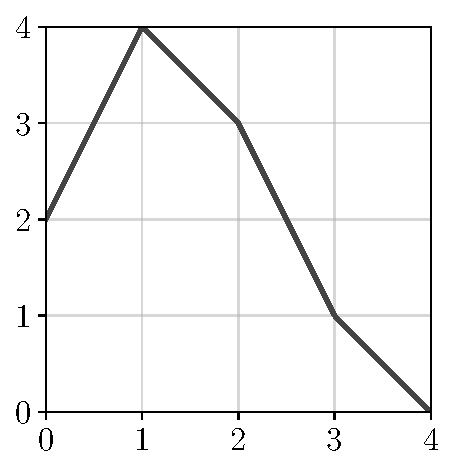
\includegraphics[width=4cm]{piecewise}
        \caption{Piecewise linear map $f$ with a period five point.}
        \label{fig:piecewise_linear}
    \end{figure}

\end{exmp}

Sharkovsky subsequently proved that topological dynamical systems over closed intervals can constructed to be of any type. In \cite{sharkovsky} he proves that you can construct maps with integer type, later in \cite{sharkovsky2} he proves you can construct maps with type in $2^\infty$. This theorem is termed Sharkovsky's Realisation Theorem and is stated below along with an elegant proof discovered by Alseda, Llibre, and Misiurewicz \cite[Section 2.2]{alm} and outlined by Burns and Hasselblatt \cite[Section 7]{burns-hasselblatt}. This insightful proof uses properties of the trunctated tent map to reveal one number in the Sharkovsky ordering at a time.

\begin{thm}[Sharkovsky's Realisation Theorem] \label{thm:sharkovsky-realisation-theorem}
    Every tail of the Sharkovsky order is the set of periods for some map f in a topological dynamical system $(I, f)$ where $I$ is a closed interval.
    \begin{proof}
        Let $([0, 1], T_h)$ a topological dynamical system, where $T_h(x) = \min(h, 1-2|x-1/2|)$ is the family of truncated tent maps with $h \in [0, 1]$, shown in Figure \ref{fig:truncated_tent}.
        
        \begin{figure}[h]
            \centering
            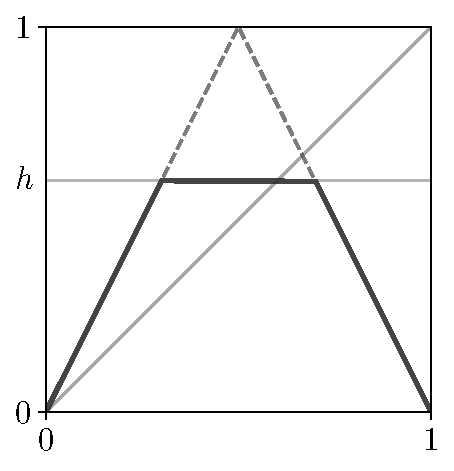
\includegraphics[width=4cm]{truncated_tent_2}
            \label{fig:truncated_tent}
            \caption{The truncated tent map $T_h$}
        \end{figure}

        It is clear that $T_0$ has only one periodic point, a fixed point at $x = 0$. However $T_1^3\left(\frac{2}{7}\right) = T_1^2\left(1-2\left\lvert\frac{2}{7} - \frac{1}{2}\right\rvert\right) = T_1^2\left(\frac{4}{7}\right) = T_1\left(1-2\left\lvert\frac{4}{7} - \frac{1}{2}\right\rvert\right) = T_1\left(\frac{6}{7}\right) = \left(1-2\left\lvert\frac{6}{7} - \frac{1}{2}\right\rvert\right) = \frac{2}{7}$. Hence $T_1$ has a period-$3$ point and so by Sharkovsky's Forcing Theorem has a periodic point for every period in the positive integers by Sharkovsky's Theorem. Hence any $k$-cycle $\mathcal{O}_{T_h}$ is also a $k$-cycle for $\mathcal O_{T_1}$ and any $k$-cycle $\mathcal{O}_{T_1}$ is also a $k$-cycle for $\mathcal{O}_{T_h}$. Now suppose $h(m) = \min \left\lbrace \max \mathcal{O}_{T_1} : \mathcal{O}_{T_1} \ \text{is $m$-cycle} \right\rbrace$. From this we can obtain that, $T_h$ has the $l$-cycle $\mathcal{O}_{T_h}$ if and only if $h(l) < h$. Moreover, $\mathcal{O}_{T_{h(m)}}$ is a $m$-cycle for $T_{h(m)}$, and all other cycles $\mathcal{O}_{T_{h(m)}}$ are contained within $[0, h(m))$. Using Sharkovsky's forcing theorem it is clear that if $m \rhd l$ then $T_{h(m)}$ has a period-$l$ orbit that lies in $[0, h(m))$ and hence $h(l) < h(m)$. Now by symmetry, $h(l) < h(m)$ if and only if $m \rhd l$. Hence we can see that for any positive integer $m$ the periodic points of $T_{h(m)}$ is the tail of the Sharkovsky order from $m \unrhd l$. Now for powers of two. By above $h(2^\infty) = \sup_k(h(2^k)) > h(2^k)$ for all $k \in \mathbb{N}$, so $T_{h(2^\infty)}$ has $2^k$-cycles for all $k \in \mathbb{N}$. Suppose $T_{h(2^\infty)}$ has an $m$-cycle with $m \neq 2^k$ for all $k \in \mathbb{N}$. Then by Sharkovsky's forcing theorem $T_{h(2^\infty)}$ has a $2m$-cycle. Because the $m$-cycle and $2m$-cycle are disjoint, at least one of them are contained in $[0, h(2^\infty))$ and hence in the interval $[0, h(2^k))$ for some $k \in \mathbb{N}$.
    \end{proof}
\end{thm}

Thus there exists a map $f$ and associated topological dynamical system $(I, f)$ such that $f$ has period-$k$ points and is of type $k$, where $k \in \mathbb{N}$ is in the Sharkovsky ordering. This concludes our study of Sharkovskys theorem and topological and symbolic relationships. In the next chapter on defining chaos we shall use the results we have developed here to prove that characteristics of chaos hold for certain topological dynamical systems.

\chapter{Defining Chaos} \label{chap:defining-chaos}
The term \emph{chaos} in Mathematics is vauge and has no universally accepted definition, hence various interpretations of chaos been invented throughout the years. As mentioned previosly, the paper \emph{'Period Three Implies Chaos'} by Li and Yorke \cite{li-yorke} first introduced the term in a mathematical context. However this paper never formally defines a notion of chaos. In subsequent years, various mathematicians have attempted to define their own interpretations of chaos. All these interpretations rely on the topological dynamical system exhibiting various defined topological characteristics. The properties relied upon by the definitions of chaos we will look at include: topological transitivity or the existence of a dense orbit, sensitive dependence on initial conditions, that perodic points are dense in the underlying metric space, and the existence of an uncountable scrambled set. In Section \ref{sec:devaney-chaos} we shall explore a widely accepted definition of chaos, termed \emph{Devaney chaos}, developed by Devaney \cite{devaney}. This definition relies upon the topological dynamical system having three properties, namely topological transitivity, sensitive dependence on initial conditions and that perodic points are dense in the underlying metric space. However, we shall show that if we have a topological dynamical system with no isolated points then the latter two properties are redundant, and are implied by topological transitivity. In Section \ref{sec:li-yorke-chaos} we shall explore \emph{Li-Yorke chaos}. This interpretation of chaos explores the types of topological dynamical systems Li and Yorke termed chaotic through the powerful definition of scrambled sets. Notably this type of chaos relies on the existence of an uncountable scrambled set. Finally in Section \ref{sec:topological-chaos} we shall study topological chaos. Topological dynamical systems that exhibit all these types of chaos will be explored. We shall see that even the trivial topological dynamical systems such as the tent map and logistic map exhibit chaos according to multiple interpretations. Before we introduce these various types of chaos however, we first need to set up some preliminary definitions.

\section{Topological Characteristics of Chaos} \label{sec:characteristics-of-chaos}

There are many different types of chaos in topological dynamical systems. All of these different types of chaos require the topologically dynamical system to display different topologically chaotic properties.
This first definition is a prime characteristic of chaotic systems. In fact we shall show later that in topological dynamical systems it is the only characteristic needed to prove that a system is chaotic in the sense of Devaney.

\begin{defn}[Topological Transitivity] \label{defn:topological-transitivity}
    Let $(X, f)$ be a topological dynamical system. The map $f$ is \emph{topologically transitive} if for every pair of non-empty open sets $U, V \subseteq X$ there exists $k > 0$ such that $f^k(U) \cap V \neq \emptyset$.
\end{defn}

Alternatively stated, in a topologically transitive mapping, points in an arbitraily small neighbourhood can be mapped to any other arbitrary neighbourhood under a repated number of iterations of the map. Hence the topological dynamical system cannot be partitioned into two disjoint non-empty open sets which are invarient under the map -- i.e.\ if $U \in X$ then $f(U) \in U$.

\begin{exmp}
    Let $(S^1, \mathcal{D})$ be the doubling map over $S^1$, where $\mathcal{D}(\theta) = 2\theta$. Let $\theta_1, \theta_2 \in S^1$. Let $(\theta_1, \theta_2) = U$ define an arc between $\theta_1$ and $\theta_2$. Suppose now $d\left(\theta_1, \theta_2\right) > \frac{2\pi}{2^k}$ for some $k \in \mathbb{N}$. Then $d\left(\mathcal{D}^k(\theta_1), \mathcal{D}^k(\theta_2)\right) = d\left( 2^k\theta_1, 2^k\theta_2 \right) = 2^k d\left( \theta_1, \theta_2 \right) > 2^k \cdot \frac{2\pi}{2^k} = 2\pi$. Hence $\mathcal{D}^k((\theta_1, \theta_2))$ covers $S^1$ so for any $V \subseteq S^1$ we obtain $\mathcal{D}^k(U) \cap V \neq \emptyset$. Hence $f$ is topologically transitive.
\end{exmp}

This next example, from \cite{kolyada-snoha}, provides a creative way of producing topologically transitive topological dynamical systems by using the orbit of any other topological dynamical system.

\begin{exmp}
    Let $(X, f)$ be a topological dynamical system and let $x \in X$ be a periodic point of $f$. Clearly $\mathcal{O}_f(x) = Y$ is finite and so $(Y, f|_y)$ is a topological dynamical system. $(Y, f|_y)$ is transitive as if $U \subseteq Y$ is open, then $f^k(U) = Y$ for some $k > 0$ and so $f^k(U) \cap V \neq 0$ for all $V \subseteq Y$ open.
\end{exmp}

This next proposition, discovered by Silverman \cite{silverman}, states that if $(X, f)$ is a topological dynamical system and $X$ has no isolated points, the existence of a dense orbit of $f$ is equivalent to $f$ being topologically transitive. In his paper, Silverman explicitly states that transitivity implies the existence of a dense orbit if $X$ is separable and second-catagory. However, since our definition of a topological dynamical system takes $X$ to be a compact metric space these propeties automatically hold. This proposition is hugely important some authors give slight variations between definitions of chaos, some definitions ask for the existence of a dense orbit and others ask for topological transitivity. Hence using this proposition we can show that these definitions are equivalent in topological dynamical systems. The proof of this proposition follows Ruette \cite[Section 2.1]{ruette}.

\begin{prop} \label{prop:dense-transitive}
    Let $(X, f)$ be a topological dynamical system and suppose $X$ has no isolated points. The map $f$ is topologically transitive if and only if there exists some $x \in X$ such that $\mathcal{O}(x)$ is dense in $X$.
    \begin{proof}
        Assume that $f$ is transitive and let $U$ be a non-empty open set. By transitivity, for every non-empty open set $V$ there exits a $k > 0$ such that $f^k(U) \cap V \neq 0$. Hence, $\bigcup_{k \geq 0}f^{-n}(U)$ is dense in $X$. As $X$ is compact, there exists a countable basis of non-empty open sets $(U_n)_{n \geq 0}$. For all $l \geq 0$, $\bigcup_{k \geq 0}f^{-k}(U_n)$ is dense by transitivity. Now define $G = \bigcap_{n \geq 0}\bigcup_{k \geq 0}f^{-k}(U_n)$. This is a dense $G_\delta$ set. If $x \in G_\delta$ then $f^k(x)$ enters any set $U_n$ for some $k$. Hence $\mathcal{O}_f(x)$ is dense in $X$. For the reverse direction let $U, V \subseteq X$ be open with $U, V \neq \emptyset$. Let $x \in X$ such that $\overline{\mathcal{O}_f(x)} = X$. Then there exists $k \in \mathbb{N}$ such that $f^k(x) \in U$. Since $X$ has no isolated points $V\, \backslash \left\lbrace f^i(x) : 0 \leq i \leq k \right\rbrace$ is open and non-empty. Hence there exists an $l \in \mathbb{N}$ such that $f^l(x) \in V\, \backslash \left\lbrace f^i(x) : 0 \leq i \leq k \right\rbrace$. Since $l > k$ and $f^l(x) = f^{l - k} \circ f^{k}(x) \in f^{l - k}(U) \cap V$ we get $f^{l - k}(U) \cap V \neq 0$. Hence $f$ is transitive.
    \end{proof}
\end{prop}

Since closed intervals have no isolated points, for topological dynamal systems $(I, f)$ where $I$ is a closed interval, topological transitivity and the existence of a dense orbit are interchangable. Note that the condition for the topological dynamical system to have no isolated points is necessary. The following is a counterexample to show the definitions are not equivalent for topological dynamical systems in general.

\begin{exmp} \label{exmp:dense-orbit-not-equal-transitive}
    Let $(X, f)$ be the topological dynamical system defined over the space $X = \left\lbrace 0 \right\rbrace \cup \left\lbrace 2^{-n} : n \in \mathbb{N} \right\rbrace$ with the standard metric, and the map $f$ where $f(0) = 0$ and $f(2^{-n}) = 2^{-n-1}$. It can be seen that $(X, d)$ is a compact space, where $d$ is the standard metric as $X$ is a closed subset of $\mathbb{R}$, containing its limit point $0$. The set $X$ contains infinitely many isolated points as we can choose $B_d(x, \varepsilon)$ around each $x = 2^{-n} \in X$ with $\varepsilon < \frac{1}{4} \min\left\lbrace 2^{-n} - 2^{-n-1}, 2^{-n + 1} - 2^{-n} \right\rbrace$ such that the open balls are disjoint and $B_d(x, \varepsilon) = \left\lbrace x \right\rbrace$. Now let $U = \left\lbrace \frac{1}{2} \right\rbrace$ and $V = \left\lbrace 1 \right\rbrace$. Then $f^k(U) = f^k(\left\lbrace \frac{1}{2} \right\rbrace) = \left\lbrace 2^{-k-1} \right\rbrace$. Hence $f^k(U) \cap V = \left\lbrace 2^{-k-1} \right\rbrace \cap \left\lbrace 1 \right\rbrace = \emptyset, \ \forall k \in \mathbb{N}$. Hence $f$ is not topologically transitive, however $\mathcal{O}(1) = \left\lbrace 1, 2^{-1}, 2^{-2}, \cdots \right\rbrace$ is dense as $\overline{\left\lbrace2^{-n}: n \in \mathbb{N}\right\rbrace} = X$.
\end{exmp}

Now lets introduce and example of a topological dynamical system with no isolated points. By Proposition \ref{prop:dense-transitive} we shall see that this max has both topological transitivty and the existence of a dense orbit.

\begin{exmp} \label{exmp:dense-orbit-and-transitive}
    In Example \ref{exmp:rigid-rotations} we introduced the rigid rotations, a topological dynamical system $(S^1, R_\alpha)$ where $R_{\alpha}(z) = ze^{i\alpha}$. Furthermore in Proposition \ref{prop:rigid-rotations-irrational} we proved that the irrational rotations gave rise to dense oribts and that these orbits where infinite. Hence $S^1$ does not contain an isolated point. Using Proposition \ref{prop:dense-transitive} we see that $(S^1, R_\alpha)$ is topologically transitive.
\end{exmp}

\begin{exmp} \label{exmp:logistic-tent-doubling-transitive}
    In Proposition \ref{prop:logisitc-tent-doubling-periodic-dense} we proved that the periodic points of the logistic map $([0, 1], F_4)$, the tent map $([0, 1], T_2)$ and the doubling map $([0, 1], D)$ are dense in $[0, 1]$. Clearly all these systems have no isolated points. Hence, using Proposition \ref{prop:dense-transitive} we can clearly see that all these maps are topologically transitive.
\end{exmp}

An important fact to note is that topological dynamical systems that are topologically transitive with an isolated point are in fact trivial, having only one periodic orbit. Hence in the rest of this text we shall restrict our study to the topological dynamical systems without an isolated point. Continuing, lets introduce our second topological characteristic of chaos, coming from Devaney \cite{devaney}.

\begin{defn}[Sensitive Dependence On Initial Conditions] \label{defn:sensitive-dependence}
    Let $(X, f)$ be a topological dynamical system and $\varepsilon > 0$. A point $x \in X$ is \emph{$\varepsilon$-unstable} if, for every neighbourhood $U$ of $x$, there exits a point $y \in U$ and $k \geq 0$ such that $d\left(f^k(x), f^k(y)\right) \geq \varepsilon$. The map $f$ has $\emph{sensitive dependence on initial conditions}$ if for all points $x \in X$, $x$ is $\varepsilon$-unstable.
\end{defn}

In other words, there exist points arbitrary close to $x$ that eventually get mapped at least $\varepsilon$ far apart under multiple applications of the map. Hence this definition states that small pertubations between iterates may eventually increase through repeated iterations of the map to become wildly different over time; behaviour which hopefully feels notionally chaotic to the reader. Note that the definition states that at least one point contained within each neighbourhood of $x$ gets mapped arbitraily far apart, not all points. Here is an example of a topological dynamical system with sensitive dependence on initial conditions.

\begin{exmp} \label{exmp:doubling-map-s1-sensitive}
    Let $(S^1, \mathcal{D})$ be the doubling map over the $S^1$, where $\mathcal{D}(\theta) = 2\theta$. Let $\theta_1, \theta_2 \in S^1$, $\varepsilon < 2^k \delta$ and suppose $d(\theta_1, \theta_2) = \delta$, then $d\left(\mathcal{D}^k(\theta_1), \mathcal{D}^k(\theta_2)\right) =  d\left(2^k\theta_1, 2^k\theta_2\right) = 2^k d(\theta_1, \theta_2) = 2^k \delta > \varepsilon$. Hence we can always choose a $k$ large enough so this holds, and so $f$ has sensitive dependence on initial conditions.
\end{exmp}

The same is true for the doubling map $([0, 1], D)$ over the unit interval. Note the example above displays a strong type of sensitive dependence on initial conditions termed expansiveness. In a topological dynamical system which exhibits expansiveness, all points arbitraily close together eventually get mapped arbitraily far apart; not just a proper subset of points as for sensitive dependence on initial conditions. We can see that the rigid rotations do not statisfy the definition of having sensitive dependence on initial conditions.

\begin{exmp} \label{exmp:rigid-rotations-not-sensitive}
    Let $(S^1, R_\alpha)$ be the rigid rotations. Let $z_1,z_2 \in S^1$, $\varepsilon > 0$ and suppose $d(z_1, z_2) < \varepsilon$, then since $R_\alpha$ is an isometry $d(R_\alpha^k(z_1), R_\alpha^k(z_2)) = d(z_1, z_2) < \varepsilon$. Hence $(S^1, R_\alpha)$ does not have sensitive dependence on initial conditions.
\end{exmp}

This concludes our study of topological characteristics of chaos. We shall now use the definitions of topological transitivity or the existence of dense orbit and sensitive dependence on initial conditions to define notions of chaos in topological dynamical systems and investigate examples of chaotic systems.

\section{Devaney Chaos} \label{sec:devaney-chaos}

Our first notion of chaos was developed by Devaney \cite{devaney} and is one of the most widely used definitions of chaos. Devaney's interpretation of chaos includes unpredictability via sensitive dependence on initial conditions, repetitive behaviour through periodic points being dense, and should be indecomposable through topological transitivity. Two characteristics which we developed in Section \ref{sec:characteristics-of-chaos}.

\begin{defn} [Devaney Chaos] \label{defn:devaney-chaos}
    A topological dynamical system $(X, f)$ is \emph{chaotic in the sense of Devaney} if it is topologically transitive, has sensitive dependence on initial conditions, and if the periodic points of $f$ are dense in $X$.
\end{defn}

The main feature of Devaney chaos is topological transitivity. After Devaney released this definition Banks et al.\ \cite{bbcds} and Glasner et al.\ \cite{glasner-weiss} showed that sensitive dependence on initial conditions is redundant. Note that this result holds even for a general mapping $f: X \to X$.

\begin{prop} \label{prop:transitivity-dense-periodic-implies-sdic}
    Let $(X, f)$ be a topological dynamical system. If the map $f$ is topologically transitive and has dense periodic points then $f$ has sensitive dependence on initial conditions.
    \begin{proof}
        Let $(X, d)$ be a metric space. Observe that we can find a $\delta_0 > 0$ such that for all $x \in X$ there exists a periodic point $q \in X$ such that $dist(\mathcal{O}_f(q), x) \geq \delta_0/2$. Proving this, take $q_1, q_2$ to be arbitrary periodic points where $\mathcal{O}_f(q_1) \cup \mathcal{O}_f(q_2) = \emptyset$. Let $\delta_0 = dist(\mathcal{O}_f(q_1), \mathcal{O}_f(q_2))$ and suppose $q_1' \in \mathcal{O}_f(q_1)$ and  $q_2' \in \mathcal{O}_f(q_2)$ are points such that $d(q_1', q_2') = \delta_0$. For all $x \in X$ either $d(q_1', x) \leq d(q_2', x)$ or by symmetry $d(q_2', x) \leq (q_1', x)$. Using the triangle inequality we find $d(q_1', q_2') \leq d(q_1', x) + d(x, q_2')$ for all $x \in X$. Hence we either have $\delta_0 = d(q_1', q_2') \leq 2d(q_1', x)$ or $\delta_0 = d(q_1', q_2') \leq 2d(q_2', x)$. Therefore we either have $dist(\mathcal{O}_f(q_1), x) \geq \delta_0/2$ or $dist(\mathcal{O}_f(q_2), x) \geq \delta_0/2$. Using this observation we can now prove $f$ has sensitive dependence on initial conditions. First let $\delta = \delta_0/8$ and let $x \in X$ be arbitrary, $x \in N$ where $N$ is an open neighbourhood. Since the periodic points of $f$ are dense in $X$ there exists a period-$n$ point $p \in U = N \cap B(x, \delta)$ open. By the observation above, there exists a periodic point $q \in X$ with $dist(\mathcal{O}_f(p), x) \geq 4\delta$. Now define $V = \bigcap_{i=0}^n f^{-i}(B(f^i(q), \delta))$. Since $V$ is a finite intersection of open sets, it itself is open. Moreover $q \in V$ so $V$ is non-empty. Since $f$ is topologically transitive, there exists a $y \in U$ with natural number $k > 0$ such that $f^k(y) \in V$. Now suppose $j = \left\lfloor \frac{k}{n} \right\rfloor + 1$ such that $1 \leq nj - k \leq n$. Hence, $f^{nj}(y) = f^{nj - k}(f^k(y)) \in f^{nj - k}(V) \subseteq B(f^{nj - k}(q), \delta)$. We also have $f^{nj}(p) = p$, so by the triangle inequality $d(f^{nj}(p), f^{nj}(y)) = d(p, f^{nj}(y)) \geq d(x, f^{nj - k}(q)) - d(f^{nj - k}(q), f^{nj}(y)) - d(p, x)$. Now as $p \in B(x, \delta)$ and $f^{nj}(y) \in B(f^{nj - k}(q), \delta)$ we have $d(f^{nj}(p), f^{nj}(y)) > 4\delta - \delta - \delta = 2\delta$. Hence, by the triangle inequality either $d(f^{nj}(x), f^{nj}(y)) > \delta$ or $d(f^{nj}(x), f^{nj}(p)) > \delta$. By definition, $f$ has sensitive dependence on initial conditions.
    \end{proof}
\end{prop}

For a general topological dynamical system this is the only superfluous property. Silverman \cite{silverman} and Vellekoop and Berglund \cite{vellekoop-berglund} later proved that for a topological dynamical system $(I, f)$ where $I$ is a closed interval, topological transitivity or equivalently the existence of a dense orbit, implies $f$ has dense periodic points in $X$. We shall introduce and later prove this result, but first we need the following lemma, which can be found here \cite[Section 4.1]{block-coppel}.

\begin{lem} \label{lem:closed-interval-no-periodic-points}
    Let $f: I \to I$ be a continuous map and $I$ an interval. Suppose $J \subseteq I$ is an interval which contains no periodic points of $f$. If $z, f^m(z), f^n(z) \in J$ where $m, n \in \mathbb{N}, \ m < n$ then either $z < f^m(z) < f^n(z)$ or $z > f^m(z) > f^n(z)$.
    \begin{proof}
        Suppose there exists a $z \in J$ such that $z < f^m(z)$ and $f^m(z) > f^n(z)$. Define $g(x) = f^m(x)$, so $z < g(z)$. If $g^{k+1}(x) < g(z)$ for some $k \in \mathbb{N}, \ n \geq 1$ then $g^k(z) - z$ has a positive value in $z$ and a negative value in $g(z)$ and by the Intermediate Value Theorem contain a point $c \in (z, g(z)) \subseteq J$ with $g^k(c) - c = 0$ and hence a $km$-periodic point. Therefore $z < g^k(z)$ for all positive integers $k$. Now let $k = n - m > 0$. Then $z < f^{(n - m)m}(z)$. Assuming $f^{(n-m)}(f^n(z)) < f^m(z)$ then taking $g = f^{n-m}(x)$ similarly yields $f^{(n-m)m}(f^m(z)) < f^m(z)$. However this results in the function $f^{(n-m)m}(x) - x$ having a positive and negative value in $f^m(z)$. Hence, by the Intermediate Value Theorem a $(n-m)m$-periodic point exits in $J$, a contradiction. The other case for $z > f^m(z) > f^n(z)$ can be proved similarly.
    \end{proof}
\end{lem}

\begin{prop} \label{prop:transitivity-interval-implies-dense-periodic}
    Let $(I, f)$ be a topological dynamical system. If the map $f$ is topologically transitive then $f$ has a dense set of periodic points.
    \begin{proof}
        We shall aim for a contradiction. Suppose that the periodic points are not dense in $I$, so there exists an interval $J \subseteq I$ where $J$ contains no periodic points. Let $x \in J$ where $x$ is not an endpoint and let $N \subsetneq J$ be a neighbourhood of $x$. Also let $E = J \ N$. Since $f$ is topologically transitive on $I$ there exists a positive integer $m$ with $f^m(N) \cap E \neq \emptyset$. Hence there exists a $y \in J$ such that $f^m(y) \in E \subsetneq J$ and since $J$ contains no periodic points $y \neq f^m(y)$. Moreover, since $f$ is continuous there exists an open neighbourhood $U$ of $y$ such that $f^m(U) \cap U \neq \emptyset$. Using topological transitivity again we can find a $n > m$ and a $z \in U$ with $f^n(z) \in U$. However then $0 < m < n$ with $z \in f^n(U)$ and $z \notin f^m(U) \implies z \leq f^n(z) \leq f^m(z)$. This is a contradiction by Lemma \ref{lem:closed-interval-no-periodic-points}. Hence the periodic points of $f$ are dense.
    \end{proof}
\end{prop}

Note that this result cannot hold generally because of the ordering over $\mathbb{R}$ used in Lemma \ref{lem:closed-interval-no-periodic-points}. Using Propositions \ref{prop:transitivity-dense-periodic-implies-sdic} and \ref{prop:transitivity-interval-implies-dense-periodic} we can clearly see that if $(I, f)$ is a topologically transitive topological dynamical system defined over an closed interval then it is chaotic in the sense of Devaney, giving us the following important result.

\begin{prop}\label{prop:chaotic-transitive}
    Let $(I, f)$ be a topological dynamical system where $I$ is a closed interval. If $f$ is topologically transitive then $(I, f)$ is chaotic in the sense of Devaney.
    \begin{proof}
        Suppose $f$ is topologically transitive. Propositions \ref{prop:transitivity-dense-periodic-implies-sdic} and \ref{prop:transitivity-interval-implies-dense-periodic} tell us that $f$ has sensitive dependence on initial conditions and the periodic points of $f$ are dense in $I$. Hence $(I, f)$ is chaotic in the sense of Devaney.
    \end{proof}
\end{prop}

As a result of this proposition, topological dynamical systems which have a topologically transitive map over a closed interval are automatically chaotic in the sense of Devaney. Here is a counterexample, proving that this result does not hold generally for topological dynamical systems.

\begin{exmp}
    Let $(S^1, R_\alpha)$ where $R_\alpha(z) = ze^{i\alpha}$ be the topological dynamical systems described by rigid rotations, except we now we shall take $\alpha$ to be solely irrational. In Example \ref{exmp:dense-orbit-and-transitive} we proved these topological dynamical systems to be topologically transitive, as irrational rotations gave rise to infinite, dense orbits. However we also proved in Example \ref{exmp:rigid-rotations-not-sensitive} that the system does not have sensitive denpendence on initial conditions. Furthermore, irrational rotations give rise to infinite orbits and so no periodic points exist. Hence we have an example of a topological dynamical system which is topologically transitive but neither has dense periodic points nor sensitive dependence on initial conditions.
\end{exmp}

The example above gives great insight into the troubles involved in trying to develop an all encompassing definition of chaos. The irrational rotations of $S^1$ have dense orbits and so are topologically transitive, but the map is not particularly interesting as nearby points are constantly mapped near together, never giving way to irratic or uncontrollable behaviour. Looking back at the definition of Devaney chaos it is clear that all of the conditions for chaos are topological and so are preserved under topological conjugate maps. This makes looking for Devaney chaotic systems much easier by the following proposition.

\begin{prop}
    Let $(X, f)$ and $(Y, g)$ be topologically conjugate, topological dynamical systems. If $f$ is chaotic in the sense of Devaney then $g$ is chaotic in the sense of Devaney.
    \begin{proof}
        By Proposition \ref{prop:transitivity-dense-periodic-implies-sdic} sensitive dependence on initial conditions was found to be redundant for topological dynamical systems. In Proposition \ref{prop:conjugacy-preserves-dense-periodic-points} we proved that if $Per(f)$ are dense in $X$ then $Per(g)$ are dense in Y. Hence we just need to prove that topological conjugacy preserves topological transitivity. Let $\varphi: X \to Y$ be a topological conjugacy between $(X, f)$ and $(Y, g)$ and suppose $f$ is topologically transitive. Let $U, V \subseteq Y$ be non-empty open sets. Since $\varphi$ is surjective $\varphi^{-1}(U)$ and $\varphi^{-1}(V)$ are non-empty. As $f$ is topologically transitive, there exits a positive integer $k > 0$ such that $f^k(\varphi^{-1}(U)) \cap \varphi^{-1}(V) \neq \emptyset$. Let $x \in \varphi^{-1}(U)$ such that $f^k(x) \in \varphi^{-1}(V)$. Now set $y = \varphi(x) \in U$ and note that $\varphi \circ f^k(x) = g^k \circ \varphi(x) = g^k(y)$. Therefore $g^k(y) = \varphi \circ f^k(x) \in V$ and so $g^k(U) \cap V \neq \emptyset$.
    \end{proof}
\end{prop}

Now lets introduce some examples of topological dynamical systems that exhibit Devaney chaos, using topological conjugacy and building on the properties we have already observed in various topological dynamical systems.

\begin{exmp}
    In Example \ref{exmp:logistic-tent-doubling-transitive} we showed that the periodic points of the logistic map $([0, 1], F_4)$, the tent map $([0, 1], T_2)$ and the doubling map $([0, 1], D)$ are all topologically transitive. By Proposition \ref{prop:chaotic-transitive} these systems are all chaotic in the sense of Devaney.
\end{exmp}

\section{Li-Yorke Chaos} \label{sec:li-yorke-chaos}

Now onto our second definition of Chaos. As mentioned in Section \ref{sec:sharkovskys-theorem-and-type}, the paper \emph{`Period Three Implies Chaos'} by Li and Yorke \cite{li-yorke} first introduced the term chaos in a mathematical context. In this paper they stated two properties of interval maps that lead to chaotic behaviour, namely sensitive dependence on initial conditions and the existence of an uncountable set with no periodic points. This was formally introduced in the following theorem.

\begin{thm} \label{thm:li-yorke-chaos-intervals}
    If $f: I \to I$ be a continuous interval map with a period three point, then there exists an uncountable set $S \subseteq I$ (cointaining no periodic points) such that, for all $x, y \in S$ where $x \neq y$
    \[\limsup_{n \to +\infty}\left\lvert f^n(x) - f^n(y) \right\rvert > 0, \ \ \ \ \liminf_{n \to +\infty}\left\lvert f^n(x) - f^n(y) \right\rvert = 0\] and for all periodic points $z \in S$ \begin{equation} \label{equ:no-assympotic-points}\limsup_{n \to +\infty}\left\lvert f^n(x) - f^n(z) \right\rvert > 0.\end{equation}
\end{thm}

Clearly by the requirement of (\ref{equ:no-assympotic-points}) in this theorem, the set $S$ contains no asymptotically stable points. Li and Yorke noted that interval maps which satisfied this equation displayed irratic and irregular behaviour. Hence within this theorem the have defined a sense of chaos in interval maps. Since this theorem was published, various authors have generalised the definition of Li-Yorke chaos to the realm of topological dynamical systems. We shall be taking the definition from Blanchard et al.\ \cite{bgsm} which uses the notion of a Li-Yorke pair, defined as follows.

\begin{defn}[Li-Yorke Pair] \label{defn:li-yorke-pair}
    Let $(X, f)$ be a topological dynamical system with $x, y \in X$ and $\delta > 0$. The pair $(x, y)$ is a \emph{Li-Yorke pair} if \[\limsup_{n \to +\infty} d\left( f^n(x) - f^n(y) \right) \geq \delta \ \ \ \text{and} \ \ \ \liminf_{n\to+\infty} d\left( f^n(x) - f^n(y) \right) = 0.\]
\end{defn}

Hence if $(x, y)$ is a Li-Yorke pair then $x$ and $y$ can be mapped at least $\delta$ far apart under multiple iterations of the map. This is the behaviour we defined, in Definition \ref{defn:sensitive-dependence}, as sensitive dependence on initial conditions. Furthermore if $(x, y)$ is a Li-Yorke pair then $x$ and $y$ can be mapped to the same point under multiple iterations of the map. In this regard we can think of iterations of these two points being scrambled amoungst the whole set $X$. Lets now define this behaviour generally over a whole set, to introduce a definition of Li-Yorke chaos

\begin{defn} [Scrambled Set, Li-Yorke Chaos] \label{defn:scrambled-set}
    A set $S \subseteq X$ is \emph{scrambled} if for all distinct $x, y \in S$, $(x, y)$ is a Li-Yorke pair. A topological dynamical system $(X, f)$ is \emph{chaotic in the sense of Li-Yorke} if there exists and uncountable scrambled set $S \subseteq X$.
\end{defn}

Note that in this general version of Li-Yorke chaos the requirement for the set $X$ to have a period three point has been excluded. Furthermore the last requirement, in (\ref{equ:no-assympotic-points}), that no points converge asymptotically to periodic points has been removed. Infact, this extra requirement makes no difference for chaos in the sense of Li-Yorke as if $S$ is a scrambled set then evey point except, at most, one point of $S$ satisfy this requirement.
\section{Topological Chaos} \label{sec:topological-chaos}

\chapter{Consequences of Chaos}

\section{Topological Entropy}
\section{Weakly Mixing Systems}


\bibliography{chaos}

\end{document}